\documentclass[11pt]{article}
\usepackage{cite}
\usepackage{graphicx}
\usepackage{amsmath}
\usepackage{tikz}
\usepackage{array}

\usepackage{pgf-pie}

\usepackage{geometry}

%\usepackage{helvet}
%\renewcommand{\familydefault}{\sfdefault}

\usepackage[strict]{changepage}
\newenvironment{subs}{\adjustwidth{3em}{0pt}}{\endadjustwidth}

\begin{document}

\begin{titlepage}
  \begin{center}
    \huge
    \textbf{ network tender report for Plymouth hotels new branch in Exeter }
    
    \vspace{1.5cm}
    \LARGE
    \textbf{Osbourne Clark}
    
    \vspace{1.5cm}
    \vspace{1.0cm}
        
    \includegraphics[width=0.4\textwidth]{./plymouthUniLogo}

    \Large
    Plymouth University\\
    United Kingdom\\
    $1^{st}$ March 2023
    
    
    
  \end{center}
\end{titlepage}

\tableofcontents

\newgeometry{left=2cm, right=2cm,bottom=2cm,top=2cm}


\begin{align*}
\text{take into account:}&\\
	&\text{Admin - 12 hosts}\\
	&\text{sales team - 20 hosts}\\
	&\text{guest network wifi - 60 hosts}\\
	&\text{employee wifi - 28 hosts}\\
	&\\
	&\text{X=6, Y=7}\\
	&\text{Network Address = 67.6.7.0/24 (classC network)}
 \end{align*}

\begin{align*}
\text{fetures of the network:}&\\
	&\text{hotel management system(view manage guest bookings)(server)}\\
	&\text{management system(view/ manage the employees’ information)(server)}\\
	&\text{web browsing for its employees(firewall policy)}\\
	&\text{web browsing for the guests(firewall policy)}\\
	&\text{web application for the guests to book room services. (server)(firewall policy)}\\
	&\text{security}
 \end{align*}

\section{introduction}
Plymouth hotel has opened a new branch in Exeter and have put out to multiple tender to create a detailed document on a proposed system and network architecture, including security aspects, for the new branch. they have supplied some requirements but are open to required additions.this report will contain a brief over view of what will added to the network, from network nodes and cabling as well as the security side, a dive into the network architecture providing detail towards ip subnetting and polices as well as the security architecture with firewalls polices.\newline
\newline
inital requirements:\newline
\begin{tabular}{||c|m{11cm}||}
\hline
	admin - &12 hosts\\
\hline
	sales team - &20 hosts\\
\hline
	guest network wifi - &60 hosts\\
\hline
	employee wifi - &28 hosts\\
\hline
	servers - & 3, hotel management system, management system(employee info), room service web application\\
\hline
	web browsing - &employees and guests\\
\hline
	future - &doubling of guest wifi in next 2 years\\
\hline
\end{tabular}\newline
\newline
additional requirements:\newline
\begin{tabular}{|c|m{11cm}|}
\hline
	demilitarized zone - &sectioning between trusted and untrusted\\
\hline
	firewalls - & between trusted and untrusted\\
\hline
	subnetting - & allow for expansion\\
\hline
	DHCP servers- & helps with expansion\\
\hline
\end{tabular}

\section{system architecture(over view of everything)}
\subsection{network}
needed features in the branch are sections of networks to allow for the zones that can be used by specifies groups, and effective topology layout for zones so little to no data collisions occur, automatic setup of new devices that are going to be connected so if expansion occurs there wont be a struggle to try to find an available IP address. 

\subsubsection{subnetting}
by subnetting, the network will be sectioned up into manageable chunks. if left unsectioned there would be no distinction from trusted devices and untrusted, and when a issue occurs on the network it would become more difficult to diagnose as there is only one switch between the outside and everything else. subnetting also allows less strain on the switches and routers that pass data , resulting in avoided collisions(data corruption), faster internet transfer speed, and reduce congestion on the network \cite{mogul1985internet}.

\subsubsection{topology (star)}
the topology is a key aspect of a network architecture as everything will need to be connected in some sort of topology. there are a range on topologyes from bus and ring to star and mesh. choosing the right one will have a massive effect on the network as it will largly effect how the data is transmitted. the ones to avoid are bus and line network as it is a half duplex connection between devices meaning only one device can transmit a message at a time, this isn't the greatest as it will significantly slow down the network and be highly prone to data collisions(corruptions). the one that i aimed for was the star topology, while still half duplex, each device will have its own collision domain so there wont be a chance of corrupted transmission due to two devices sending data. star topology allows for easy scalability and has good performance for transmission\cite{bisht2015analytical}.

\subsubsection{physical devices connection}
1Gb cable will be used to transfer data between routers and switches so data can flow fast from network to network or from network to the outer internet. this will help congestion if it occurs as the data will be quickly forwarded allowing for the the routers and switches internal queue to empty for new data to be received and transmitted. 10Mb Ethernet will be used to transfer data from host to switch as this connection doesn't need to be fast as there wont be big amount of data being passed at one time. 10Mb Ethernet will also be used to connect the employees and guests wireless access point to the respected switches.

\subsubsection{automatic ip assigning (DHCP)}
DHCP(dynamic host configuration protocol) servers for the networks will be very useful especially on the employee and guest wifi due the the plug and play functionality, meaning devices can then connect without needing their ip addresses set up manually. it could be a issue to pin down a problem if a problem occurs inside the network but it does also layout clear lines on were a network start and stops. by using DHCP, expansion will be easier as each new pc connected will be automatically assigned a ip and with this approach expansion will be possible in the guest network, employee network, admins network and sales network\cite{droms1999automated}.

\subsection{security}
security aspects will be put in place to both separate and limit the data transmission through the network. this will stop nuisance outside IP addresses from entering the trusted network, this would also stop ip address from the untrusted network section from accessing the trusted area. the separation will keep public facing and untrusted sources from accessing trusted resources such as employee information.

\subsubsection{firwalls}
firewalls will be put in place just before entering the intranet as well as just before entering the trusted network. by having two separate entrances two different sets of fire wall policies can be put in place, this can allow for forwarding request to web servers but not let them into other aspects of the network. firewalls will block other aspects, such as port designated for specific purposes like ftp and and ssh, this is so untrusted sources cant take advantage of them like constructing a tunnel to the outside that would allow unknown entities in \cite{ioannidis2000implementing}.

\subsubsection{demilitrization zone}
demilitarization zone will be put in to further serpate the networks into trusted and untrusted. demilitarization zone has already be summed up in the firewalls section in system architecture. it will allow for two separate firewall polices to be defined to add two layers of protection for the most valuable aspects of the network. the guest wireless accesses point will be in the untrusted section as well as the public facing servers such as the room service server. this will keep important aspects safe and make sure sensitive information can be kept away from public knowledge\cite{webb2014network}.

\section{network architecture(detailed view)}
\subsection{subnetting layout}
the subnet will be laid out into seven subnets: guest, staff, sales team, admin, public side servers, between routers, and private servers.\newline
 guest network will take up half of the address space as they have said they plan to increase its capacity of its connections in the next two years. admin, sales team and staff will take up one eight each, this will also allow for expansion in each subnet if needed. private servers will take up one sixteenths, if there are more servers needed then adding them wont be any trouble but its  on a smaller subnet as most of the main servers have already been specified. between routers subnet and public side servers will take up one thirtytwoths each, only one subnet between routers are needed and there isn't a reason to add more at the moment. only one server is currently connected to public side. 
\begin{figure}[!hbt]
	\begin{center}
	  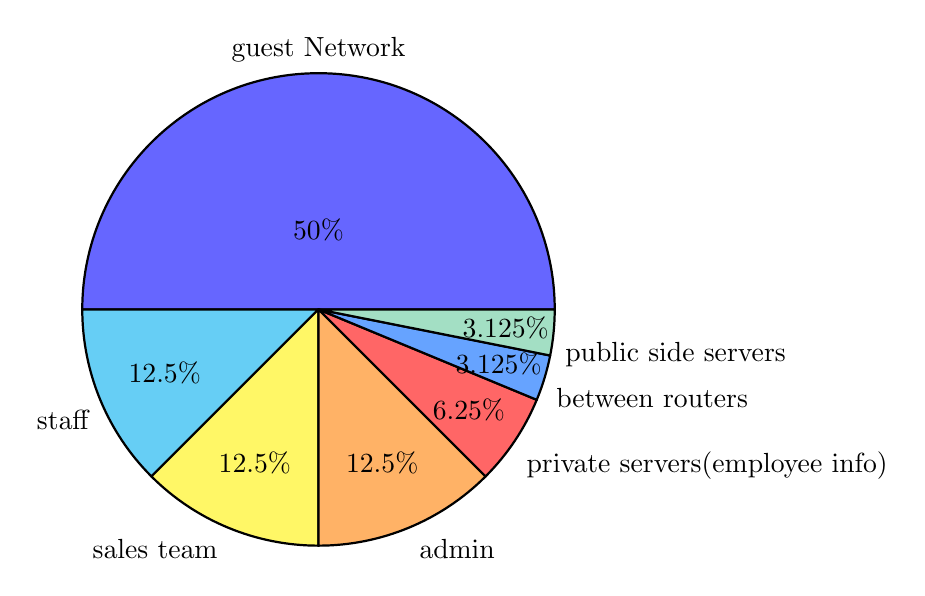
\begin{tikzpicture}
    	    \pie{50/guest Network, 12.5/staff, 12.5/sales team, 12.5/admin, 6.25/private servers(employee info), 3.125/between routers, 3.125/public side servers}
	  \end{tikzpicture}
	\end{center}
	\caption{current seperation of ip address space}
\end{figure}

\begin{center}
\begin{table}[!hbt]
	ID = 10777267 x = 6 y=7\newline
	Network = 67.6.7.0/24\newline
	\begin{tabular}{|c|c|c|c|c|}
	\hline
		network ID		               &guest                 &staff                 &sales team           &admin          \\
	\hline
		No. subnet Bits                  &25                     &27                    &27                        &27         \\
	\hline
		subnet mask$_{10}$          &255.255.255.128&255.255.255.224&255.255.255.224  &255.255.255.224            \\
	\hline
		No. usable subnets             &2                      &8                       &8                        &8          \\
	\hline
		No. usable hosts per subnet&126                   &30                     &30                       &30    \\
	\hline
		network address                &67.6.7.0            &67.6.7.224         &67.6.7.192           &67.6.7.128       \\
	\hline
		first host                           &67.6.7.1            &67.6.7.225         &67.6.7.193          &67.6.7.129        \\
	\hline
		last host                            &67.6.7.126        &67.6.7.254        &67.6.7.222           &67.6.7.158       \\
\hline
\hline
	\end{tabular}
	\begin{tabular}{|c|c|c|c|}
	\hline
		network ID		                                &private servers                 &between routers  &public servers\\
	\hline
		No. subnet Bits                                      &28                                  &29                      &29\\
	\hline
		subnet mask$_{10}$            &255.255.255.240              &255.255.255.248 &255.255.255.248\\
	\hline
		No. usable subnets                                  &16                                   &32                     &32\\
	\hline
		No. usable hosts per subnet                    &14                                   &6                       &6\\
	\hline
		network address                         &67.6.7.160                       &67.6.7.176         &67.6.7.184\\
	\hline
		first host                                   &67.6.7.161                       &67.6.7.177         &67.6.7.185\\
	\hline
		last host                                    &67.6.7.174                       &67.6.7.182          &67.6.7.190\\
	\hline
	\end{tabular}
	\caption{infomation on designated subnets}
\end{table}
\end{center}

\subsection{topology (star) acn device connection cables}
the topology being used is a star and completely removes the possibility of collisions. while it eliminates collisions it is more expensive as other simpler topology such as bus  where the computers are connected with only one Ethernet cable. this topology is specifically chosen for cable connected devices such as the admin and sales teams as well as the servers, but is unnecessary to choose for the WAPs(wireless access points) as the act as hubs. router to router, router to switch and switch to switch will all have one Gb cables connecting them so little congestion occurs, but host to switch including server to switch will have fast ten Mb cables as only on device will be communicating on the line, this will also reduce the cost.


\begin{figure}[!hbt]
 	\begin{center}
	  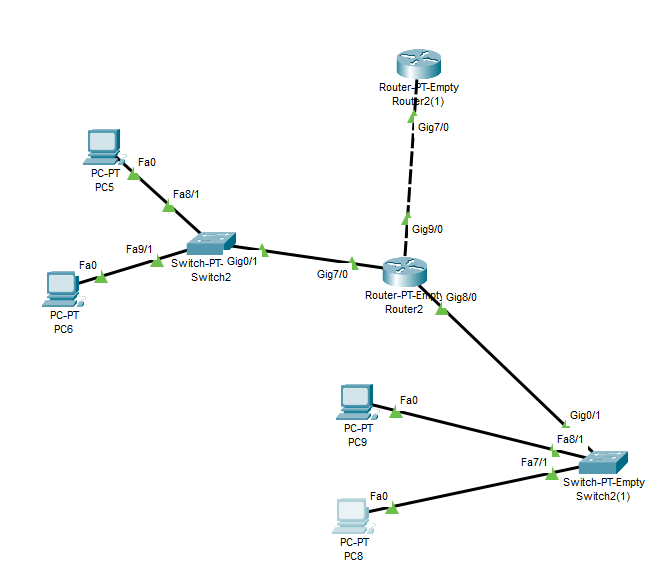
\includegraphics[width=0.4\textwidth]{./simpleExample}
	\end{center}
	\caption{a simple example of the connectivity between routers, switches and hosts and how a star newrok is layed out}
\end{figure}


\subsection{DHCP and DNS servers}
there will be 2 DHCP(dynamic host configuration protocol) servers, one between the guest and staff wifi, another between the admin and sales team networks. only one of the DHCP servers are needed that being on the staff and guest wifi as this will allow automatic IP assignment to guest without needing IT intervention. the device currently between the admin and sales team networks is more of a quality of life device as computers that are newly connected or swapped out wont need manual setup, but if a low cost is wanted this server can be removed and the computers just need to be connected manually. 
only one DNS(domain name service) server will be used and will be located on the guest wifi network, this will allow for the guests to not need to remember an IP address to connect to the room service server. this will also stop outside ip address from connecting to the room service servers, so people who aren't staying at the hotel cant request room service.

\subsection{routers and switches}
there will be 2 routers and 11 switches. the 2 routers will be mandatory to implement as this will section up the trusted from untrusted zones. the 11 switches can be cut down to 6 if needed for cost reasons, there are extra for the admin and sales teams networks so all computers aren't send to and receiving from one switch and potentially overloading the sending and receiving queues. both routers have static routes to each side of the network, the firewall policies will filter out unwanted packets.

\subsection{servers}
there are 3 servers, the server with employee information and guest bookings server will be on the trusted side of the demilitarized zone while the room service server will be on the untrusted side. the room service server will be on this side to allow for guests to connect to the room booking service though the public IP address or the domain name attached to it.

\section{cyber security architecture}
\subsection{firewall policies}
currently these are the firewall policies that will be put in place. they will allow all the sub networks to accesses the internet though port 80 as the destination and any port above 49,151 as the source but will block all other communication on all other ports on both TCP and UDP. this is that same for all subnets, the employee policies will be slightly different to allow for connection to the private servers such as the employees info and room booking.

\begin{table}[!hbt]
	\begin{tabular}{|c|c|c|c|c|c|}
	\hline		
		permit or deny		 &Permit	&Permit	&Deny&Deny&Deny\\ 
	\hline
		Protocol(udp tcp)	&Tcp	&Tcp	&Tcp&Udp&Udp\\
	\hline
		Src			&67.6.7.0/25	&Any	&67.6.7.0/25&67.6.7.0/25&Any\\
	\hline
		src Reverse Mask	&0.0.0.127	&	&0.0.0.127&0.0.0.127&\\
	\hline
		src Port		&49,151(greater than)	&80	&all&all&all\\	
	\hline
		dest			&any	&67.6.7.0/25	&any&any&67.6.7.0/25\\
	\hline
		dest Reverse Mask	&	&0.0.0.127	&&&0.0.0.127\\
	\hline
		dest port		&80	&49,151(greater than)	&all&all&all\\
	\hline
		int or out		&out	&In	&out&Out&In\\
	\hline
		description		&Out to internet	&In from internet	&	&	&\\
	\hline
	\end{tabular}
	\caption{Guest  policys}
\end{table}
\begin{table}[!hbt]
\adjustwidth{-1cm}{0pt}
	\begin{tabular}{|c|c|c|c|c|c|}
	\hline		
		permit/dent		 &Permit	&Permit	&Deny	&Deny	&Deny\\ 
	\hline
		Protocol(udp tcp)	&Tcp	&Tcp	&Tcp	&Udp	&Udp\\
	\hline
		Src			&67.6.7.192/27	&Any	&67.6.7.192/27	&67.6.7.192/27	&Any\\
	\hline
		src Reverse Mask	&0.0.0.31	&	&0.0.0.31	&0.0.0.31	&\\
	\hline
		src Port		&49,151 (greater than)	&80	&all	&all	&all\\	
	\hline
		dest			&any	&67.6.7.192/27	&any	&any	&67.6.7.192/27\\
	\hline
		dest Reverse Mask	&	&0.0.0.31	&	&	&0.0.0.31\\
	\hline
		dest port		&80	&49,151 (greater than)	&all	&all	&all\\
	\hline
		int or out		&out	&In	&out	&Out	&In\\
	\hline
		description		&Out to internet	&In from internet	&	&	&\\
	\hline
	\end{tabular}
\endadjustwidth
	\caption{sales team policys}

\end{table}
\begin{table}[!hbt]
%\adjustwidth{-1cm}{0pt}
	\begin{tabular}{|c|c|c|c|c|}
	\hline		
		permit/dent		 &Permit	&Permit	&Permit&Permit\\ 
	\hline
		Protocol(udp tcp)	&Tcp	&Tcp	&Tcp&Tcp\\
	\hline
		Src			&67.6.7.224/27	&any	&67.6.7.160/28&67.6.7.224/27\\
	\hline
		src Reverse Mask	&0.0.0.31	&&0.0.0.15&0.0.0.31\\
	\hline
		src Port		&49,151 (greater than)	&80	&all&all\\	
	\hline
		dest			&Any	&67.6.7.224/27	&67.6.7.224/27&67.6.7.160/28\\
	\hline
		dest Reverse Mask	&	&0.0.0.31	&0.0.0.31&0.0.0.15\\
	\hline
		dest port		&80	&49,151 (greater than)	&all&all\\
	\hline
		int or out		&out	&In	&In	&Out\\
	\hline
		description		&Out to internet	&In from internet	&From private servers	&To private servers 	\\
	\hline
	\hline	
	\end{tabular}
	\begin{tabular}{|c|c|c|c|}
	\hline		
		permit/dent		 &Deny&Deny&Deny\\ 
	\hline
		Protocol(udp tcp)	&Tcp&Udp&Udp\\
	\hline
		Src			&67.6.7.224/27&67.6.7.224/27&Any\\
	\hline
		src Reverse Mask	&0.0.0.31&0.0.0.31&\\
	\hline
		src Port		&all&all	&all\\	
	\hline
		dest			&Any&Any&67.6.7.224/27\\
	\hline
		dest Reverse Mask	&&	&0.0.0.31\\
	\hline
		dest port		&all&all&all\\
	\hline
		int or out		&Out	&Out	&In\\	
	\hline
		description		&&&\\
	\hline
	\end{tabular}
%\endadjustwidth
	\caption{Employee wifi policys}
\end{table}
\begin{table}[!hbt]
\adjustwidth{-1cm}{0pt}
	\begin{tabular}{|c|c|c|c|c|c|}
	\hline		
		permit/dent		 &Permit	&Permit	&Deny&Deny&Deny\\ 
	\hline
		Protocol(udp tcp)	&Tcp	&Tcp	&Tcp&Udp&Udp\\
	\hline
		Src			&67.6.7.128/27	&Any	&67.6.7.128/27&67.6.7.128/27&Any\\
	\hline
		src Reverse Mask	&0.0.0.31	&	&0.0.0.31&0.0.0.31&\\
	\hline
		src Port		&49,151 (greater than)	&80	&all&all&all\\	
	\hline
		dest			&any	&67.6.7.128/27	&any&any&67.6.7.128/27\\
	\hline
		dest Reverse Mask	&	&0.0.0.31	&&&0.0.0.31\\
	\hline
		int or out		&out	&In	&out	&Out	&In\\
	\hline
		dest port		&80	&49,151 (greater than)	&all&all&all\\
	\hline
		description		&Out to internet	&In from internet	&	&	&\\
	\hline
	\end{tabular}
\endadjustwidth
	\caption{admin polices}


\end{table}

\subsection{demilitarization zone}
there will be a demilitarized zone to separate the trusted from untrusted. it will be laid out as followed: guest network and the public side server on the untrusted side, this means the guests wont be able to access or communicate with the private servers (employee info server and guest bookings server), or with admin, sales team and staff computers.


\section{conclusions  }
this report has laid out the network that will be implemented taking into account the requirements layout by Plymouth hotel along with additional requirements and some extra quality of life features. 
the connecting cables that will be used take into account for high speed internet by using 1gb cables for switch and router connections, if cost is a something Plymouth hotel is wanting to keep down they can be downgraded to 10mb instead for all of the Ethernets. all but 6 of the physical devices are needed, there are extra for both convenience and to not overload a single switch if high traffic occurs. the extra device that isn't needed is the admin and sales team DHCP server, this is there to only make connecting devices more easy. IP addresses have been laid out to allow for expandability as well as to show clear distinctions between sections of the entire network. while all networks have the available capacity for the required devices, if major expansion occur the IP addresses will need reconfiguring. firewall have been put in place to block the unwanted traffic. . while all spesifyed policies have been put inplace such as connection to the internet, re configuration might need to to allow for other protocols such as ssh and ftp if needed. this is the best for expandability as well as ease of setup. if a cheaper solution is required some extra hardware can be removed, and cables be downgraded to reduce the costs.

\bibliography{references.bib}
\bibliographystyle{plain}


\restoregeometry


\end{document}